\documentclass[14pt]{beamer}
\title[COJ:Java:01]{COJ :: Packages \& Access Modifiers}
\author[TS]{TalentSprint}
\institute[L\&D]{Licensed To Skill}
\date{Version 1.0.4}
\usefonttheme{serif}
\usecolortheme{orchid}
\usepackage{bookman}
\usepackage{hyperref}
\usepackage[T1]{fontenc}
\usepackage{graphicx}
\usepackage{listings}
\graphicspath{{../../Images/}}
\beamertemplateballitem
\usebackgroundtemplate{
\includegraphics[width=\paperwidth]{TS-Logo.jpg}}
\lstset{language=Java,numbers=left, numberstyle=\tiny, numbersep=10pt, showstringspaces=false, breaklines=true,keepspaces=true, columns=flexible}
\begin{document}

\begin{frame}
  \titlepage
\end{frame}

\begin{frame}{Learning Objectives}
The content in this presentation is aimed to learn the following:
  \begin{itemize}
  \item Understanding Packages
  \item Types of Packages
  \item Usage of packages
  \item Working with predefined and user defined packages
  \item Use access modifier 
  \item Explain the scope of various access modifiers
  \end{itemize}
\end{frame}

\begin{frame}{Packages}
What is a Package?

A package is a grouping of related types (classes, interfaces, Exceptions and Annotations) providing access protection and Name Space Management.
\begin{tabular}{l l}
\begin{minipage}{0.25\textwidth}

\includegraphics[scale=.4]{built-in-packages.png}
\end{minipage}
&
\begin{minipage}{0.65\textwidth}
Built-In packages are library packages.
  Example: java.lang, java.awt etc.
\end{minipage}
\end{tabular}

\begin{tabular}{l l}
\begin{minipage}{0.25\textwidth}
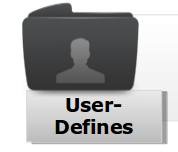
\includegraphics[scale=.4]{user-defines-packages.png}
\end{minipage}
&
\begin{minipage}{0.65\textwidth}
User-defined packages are user developed packages.
\end{minipage}
\end{tabular}
\end{frame}

\begin{frame}{Why Packages}
\begin{figure}[H]
 \begin{center}
   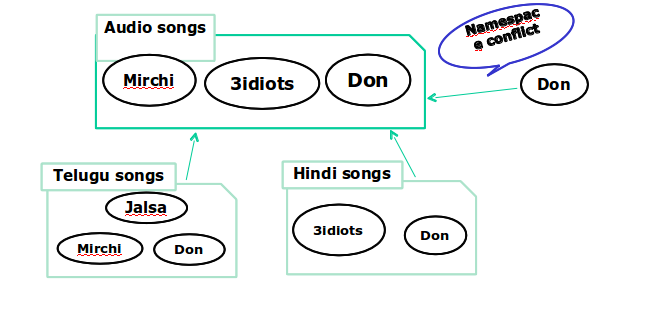
\includegraphics[scale=.4]{why-packages.png}
 \end{center}
 \end{figure}
\end{frame}

\begin{frame}{Packages}
\texttt{Why Packages?}
\begin{itemize}
 \item Using packages programmers can easily determine that these types are related.
 \item As packages follow naming conventions, a programmer knows that all graphical related methods will be present in a package named graphics.
 \item The names of your types won't conflict with the type names in other packages because the package creates a new namespace.
\end{itemize}


\end{frame}

\begin{frame}[fragile]{Packages}
\texttt{Creating Packages}
\begin{block}{Syntax to create a package:}
\lstinline!package packagename;!
\end{block}
Here package is a keyword used to create a package followed by packagename.
\end{frame}
\begin{frame}{Packages}
\texttt{Creating sub packages}
\begin{block}{Syntax to create a sub-package:}
\lstinline!package package1.package2;!
\end{block}
Here package1 is a package, which contains a sub-package named package2.
\begin{block}{Note}
The package statement must be the first line in the source file.
\end{block}
\end{frame}


\begin{frame}[fragile]{Packages}
\texttt{Program to demonstrate packages:}
\begin{lstlisting}[numbers=none]
package mypackage;
public class HelloWorld {
    public static void main(String[] args) {
        System.out.println("Hello World");
    }
}
\end{lstlisting}
\end{frame}

\begin{frame}{Packages}
\begin{block}{How to compile the above program:}
javac -d . HelloWorld.java
\end{block}
\begin{itemize}
 \item ``-d'' stands for ``directory'' which explains the compiler the location where the class files should be created.
 \item  .(dot) stands for the current directory.
\end{itemize}
\end{frame}

\begin{frame}{Packages}
\texttt{What happens when we use package statement?} 
\begin{itemize}
 \item When we use a package statement, the underlying operating system will create a directory  with the same name of the package.
 \item As a programmer we should make sure that the \lstinline!.class! files should be compiled to the same package directory.
\end{itemize}
Make sure that you set the CLASSPATH to the directory where the \lstinline!.class! files are located. After setting the classpath, we can run our programs as follows:

\textbf{java packagename.classname }
\end{frame}


\begin{frame}{Packages}
 \texttt{Using Packages?}
 
 Import statement is used to get access to the classes present in packages.
 \texttt{Importing a Single Package Member:}
 \begin{block}{Syntax}
  \lstinline!import packagename.Classname;!
 \end{block}
While importing the packages we need to mention the fully qualified package name as below.
\begin{block}{Example}
 \lstinline!import java.lang.Integer;!
\end{block}
\end{frame}

\begin{frame}{Packages}
 \texttt{Importing an Entire Package:}
 
 We can access multiple classes present in the same package using single import statement as follows: 
 \begin{block}{Syntax:}
 \lstinline!import packagename.subpackage.*;! 
 \end{block}
 Asterisk(*) represents all the classes present in that package.
 \begin{block}{Example:}
  \lstinline!import java.lang.*;!
 \end{block}
 \end{frame}
 
 \begin{frame}{Packages}
  While importing the packages we need to mention the fully qualified package name as above.
\begin{block}{Note}
 It is a good programming practice to mention the fully qualified name of number of classes which are  accessed from the same package. 
\end{block}
\begin{block}{Example}
 \lstinline!import java.lang.Integer;!
 \lstinline!import java.lang.Double;!
\end{block}
\end{frame}

\begin{frame}{Packages}
 \textbf{Points to remember}	
 
 The industry convention for creating a user-defined package is called as \texttt{Reverse Domain Naming Convention principle}.
 \begin{block}{Syntax and Example}
  \lstinline!package domainname.companyname.projectname.modulename;!
  \lstinline!package com.talentsprint.osp.inventory;!
 \end{block}
To access the sub-package classes one has to explicitly import it.
\lstinline!import javax.servlet.*;!
\lstinline!import javax.servlet.http.*;!
\end{frame}

\begin{frame}{Access Modifier}
 \begin{tabular}{l l}
\begin{minipage}{0.1\textwidth}

\includegraphics[scale=.4]{Access-Specifiers.png}
\end{minipage}
&
\begin{minipage}{0.85\textwidth}
Access specifiers specifies who can access them. There are four access specifiers used in java.
\end{minipage}
\end{tabular}
\begin{figure}[H]
 \begin{center}
   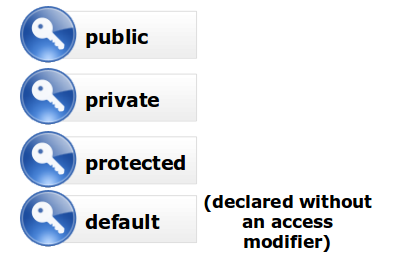
\includegraphics[scale=.3]{list-access-specifier.png}   
 \end{center}
  \end{figure}
Access Specifiers regulates the access to classes, constructors, methods and fields.
  \end{frame}

\begin{frame}{Access Modifier}

 \texttt{Access modifiers are restricted to two levels:}
 
 \begin{tabular}{l l}
\begin{minipage}{0.1\textwidth}

\includegraphics[scale=.4]{class-level-access-specifier.png}
\end{minipage}
&
\begin{minipage}{0.85\textwidth}
Class level access specifiers
\end{minipage}
\end{tabular}
 
\begin{tabular}{l l}
\begin{minipage}{0.1\textwidth}

\includegraphics[scale=.4]{member-level-access-specifier.png}
\end{minipage}
&
\begin{minipage}{0.85\textwidth}
Member level access specifiers
\end{minipage}
\end{tabular} 
\end{frame}

\begin{frame}{Access Modifier}
 \texttt{Access modifiers are restricted to two levels:}
 \begin{figure}[H]
 \begin{center}
   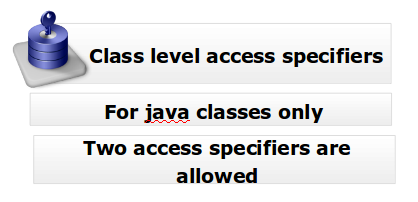
\includegraphics[scale=.3]{class-level-description.png}   
 \end{center}
  \end{figure}
  
  \begin{tabular}{l l}
\begin{minipage}{0.15\textwidth}

\includegraphics[scale=.4]{public.png}
\end{minipage}
&
\begin{minipage}{0.85\textwidth}
Can be accessed from anywhere
\end{minipage}
\end{tabular} 

\begin{tabular}{l l}
\begin{minipage}{0.25\textwidth}

\includegraphics[scale=.5]{default.png}
\end{minipage}
&
\begin{minipage}{0.75\textwidth}
Can only be accessed from `same package'.
\end{minipage}
\end{tabular} 
\end{frame}

\begin{frame}{Access Modifier}
 \texttt{Access modifiers are restricted to two levels:}
 \begin{tabular}{l l}
\begin{minipage}{0.1\textwidth}

\includegraphics[scale=.4]{member-level-access-specifier.png}
\end{minipage}
&
\begin{minipage}{0.85\textwidth}
Member level access specifiers
\end{minipage}
\end{tabular} 
\begin{itemize}
 \item For java variables and java methods
 \item All four access specifiers are allowed
\end{itemize}
\begin{figure}[H]
 \begin{center}
   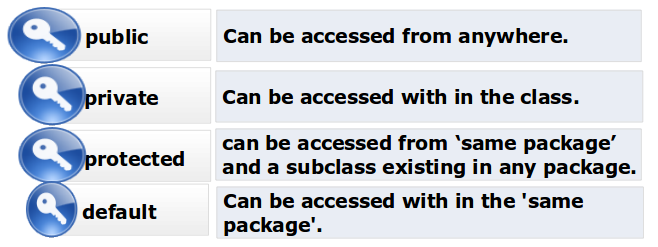
\includegraphics[scale=.3]{public-private-protected-default.png}   
 \end{center}
  \end{figure}
\end{frame}

\begin{frame}{Access Modifier}
 \texttt{Tabular formulation of member level access:}
 \begin{tabular}{l l}
\begin{minipage}{0.1\textwidth}

\includegraphics[scale=.4]{member-level-access-specifier.png}
\end{minipage}
&
\begin{minipage}{0.85\textwidth}
Member level access specifiers
\end{minipage}
\end{tabular} 
\begin{figure}[H]
 \begin{center}
   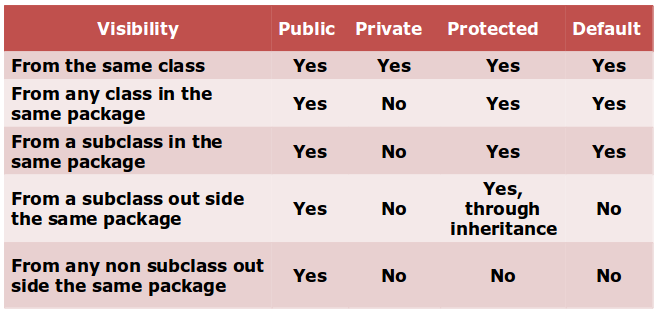
\includegraphics[scale=.4]{access-specifiers-table.png}   
 \end{center}
  \end{figure}
\end{frame}

\begin{frame}{Access Modifier}
 \begin{figure}[H]
 \begin{center}
   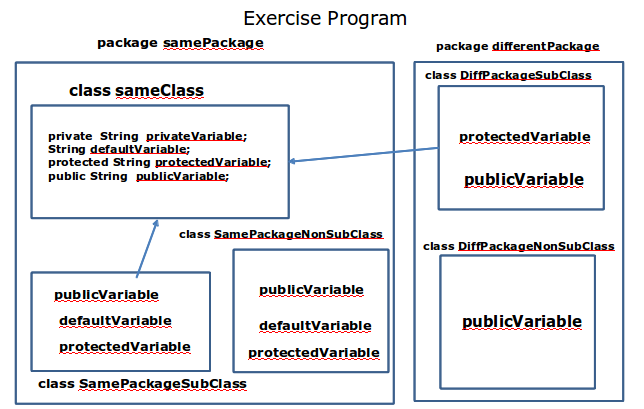
\includegraphics[scale=.4]{exercise-program.png}   
 \end{center}
  \end{figure}
\end{frame}


\begin{frame}{Packages and Access Modifiers}
 \begin{figure}[H]
 \begin{center}
   
\includegraphics[scale=.3]{qa.png}   
 \end{center}
  \end{figure}
\end{frame}

\end{document}
